% Template for PLoS
% Version 3.6 Aug 2022
%
% % % % % % % % % % % % % % % % % % % % % %
%
% -- IMPORTANT NOTE
%
% This template contains comments intended 
% to minimize problems and delays during our production 
% process. Please follow the template instructions
% whenever possible.
%
% % % % % % % % % % % % % % % % % % % % % % % 
%
% Once your paper is accepted for publication, 
% PLEASE REMOVE ALL TRACKED CHANGES in this file 
% and leave only the final text of your manuscript. 
% PLOS recommends the use of latexdiff to track changes during review, as this will help to maintain a clean tex file.
% Visit https://www.ctan.org/pkg/latexdiff?lang=en for info or contact us at latex@plos.org.
%
%
% There are no restrictions on package use within the LaTeX files except that no packages listed in the template may be deleted.
%
% Please do not include colors or graphics in the text.
%
% The manuscript LaTeX source should be contained within a single file (do not use \input, \externaldocument, or similar commands).
%
% % % % % % % % % % % % % % % % % % % % % % %
%
% -- FIGURES AND TABLES
%
% Please include tables/figure captions directly after the paragraph where they are first cited in the text.
%
% DO NOT INCLUDE GRAPHICS IN YOUR MANUSCRIPT
% - Figures should be uploaded separately from your manuscript file. 
% - Figures generated using LaTeX should be extracted and removed from the PDF before submission. 
% - Figures containing multiple panels/subfigures must be combined into one image file before submission.
% For figure citations, please use "Fig" instead of "Figure".
% See http://journals.plos.org/plosone/s/figures for PLOS figure guidelines.
%
% Tables should be cell-based and may not contain:
% - spacing/line breaks within cells to alter layout or alignment
% - do not nest tabular environments (no tabular environments within tabular environments)
% - no graphics or colored text (cell background color/shading OK)
% See http://journals.plos.org/plosone/s/tables for table guidelines.
%
% For tables that exceed the width of the text column, use the adjustwidth environment as illustrated in the example table in text below.
%
% % % % % % % % % % % % % % % % % % % % % % % %
%
% -- EQUATIONS, MATH SYMBOLS, SUBSCRIPTS, AND SUPERSCRIPTS
%
% IMPORTANT
% Below are a few tips to help format your equations and other special characters according to our specifications. For more tips to help reduce the possibility of formatting errors during conversion, please see our LaTeX guidelines at http://journals.plos.org/plosone/s/latex
%
% For inline equations, please be sure to include all portions of an equation in the math environment.  For example, x$^2$ is incorrect; this should be formatted as $x^2$ (or $\mathrm{x}^2$ if the romanized font is desired).
%
% Do not include text that is not math in the math environment. For example, CO2 should be written as CO\textsubscript{2} instead of CO$_2$.
%
% Please add line breaks to long display equations when possible in order to fit size of the column. 
%
% For inline equations, please do not include punctuation (commas, etc) within the math environment unless this is part of the equation.
%
% When adding superscript or subscripts outside of brackets/braces, please group using {}.  For example, change "[U(D,E,\gamma)]^2" to "{[U(D,E,\gamma)]}^2". 
%
% Do not use \cal for caligraphic font.  Instead, use \mathcal{}
%
% % % % % % % % % % % % % % % % % % % % % % % % 
%
% Please contact latex@plos.org with any questions.
%
% % % % % % % % % % % % % % % % % % % % % % % %

\documentclass[10pt,letterpaper]{article}
\usepackage[top=0.85in,left=2.75in,footskip=0.75in]{geometry}

% amsmath and amssymb packages, useful for mathematical formulas and symbols
\usepackage{amsmath,amssymb}

% Use adjustwidth environment to exceed column width (see example table in text)
\usepackage{changepage}

% textcomp package and marvosym package for additional characters
\usepackage{textcomp,marvosym}

% cite package, to clean up citations in the main text. Do not remove.
\usepackage{cite}

% Use nameref to cite supporting information files (see Supporting Information section for more info)
\usepackage{nameref,hyperref}

% line numbers
\usepackage[right]{lineno}

% ligatures disabled
\usepackage[nopatch=eqnum]{microtype}
\DisableLigatures[f]{encoding = *, family = * }

% color can be used to apply background shading to table cells only
\usepackage[table]{xcolor}

% array package and thick rules for tables
\usepackage{array}

% add by Z
\usepackage{booktabs}
\usepackage{multirow}
\usepackage{tabularx}

% create "+" rule type for thick vertical lines
\newcolumntype{+}{!{\vrule width 2pt}}

% create \thickcline for thick horizontal lines of variable length
\newlength\savedwidth
\newcommand\thickcline[1]{%
  \noalign{\global\savedwidth\arrayrulewidth\global\arrayrulewidth 2pt}%
  \cline{#1}%
  \noalign{\vskip\arrayrulewidth}%
  \noalign{\global\arrayrulewidth\savedwidth}%
}

% \thickhline command for thick horizontal lines that span the table
\newcommand\thickhline{\noalign{\global\savedwidth\arrayrulewidth\global\arrayrulewidth 2pt}%
\hline
\noalign{\global\arrayrulewidth\savedwidth}}


% Remove comment for double spacing
%\usepackage{setspace} 
%\doublespacing

% Text layout
\raggedright
\setlength{\parindent}{0.5cm}
\textwidth 5.25in 
\textheight 8.75in

% Bold the 'Figure #' in the caption and separate it from the title/caption with a period
% Captions will be left justified
\usepackage[aboveskip=1pt,labelfont=bf,labelsep=period,justification=raggedright,singlelinecheck=off]{caption}
\renewcommand{\figurename}{Fig}

% Use the PLoS provided BiBTeX style
\bibliographystyle{plos2015}

% Remove brackets from numbering in List of References
\makeatletter
\renewcommand{\@biblabel}[1]{\quad#1.}
\makeatother



% Header and Footer with logo
\usepackage{lastpage,fancyhdr,graphicx}
\usepackage{epstopdf}
%\pagestyle{myheadings}
\pagestyle{fancy}
\fancyhf{}
%\setlength{\headheight}{27.023pt}
%\lhead{\includegraphics[width=2.0in]{PLOS-submission.eps}}
\rfoot{\thepage/\pageref{LastPage}}
\renewcommand{\headrulewidth}{0pt}
\renewcommand{\footrule}{\hrule height 2pt \vspace{2mm}}
\fancyheadoffset[L]{2.25in}
\fancyfootoffset[L]{2.25in}
\lfoot{\today}

%% Include all macros below

\newcommand{\lorem}{{\bf LOREM}}
\newcommand{\ipsum}{{\bf IPSUM}}

%% END MACROS SECTION


\begin{document}
\vspace*{0.2in}

% Title must be 250 characters or less.
\begin{flushleft}
{\Large
\textbf\newline{?? Multicolumnar model finds gamma oscillation beyond winner-takes-all strategy in visual attention} % Please use "sentence case" for title and headings (capitalize only the first word in a title (or heading), the first word in a subtitle (or subheading), and any proper nouns).
}
\newline
% Insert author names, affiliations and corresponding author email (do not include titles, positions, or degrees).
\\
Tianyi Zheng\textsuperscript{1\Yinyang},
Masato Sugino\textsuperscript{1\Yinyang},
Yasuhiko Jimbo\textsuperscript{1},
G. Bard Ermentrout\textsuperscript{2},
Kiyoshi Kotani\textsuperscript{3},
\\
\bigskip
\textbf{1} Department of Precision Engineering, The University of Tokyo, Tokyo, Japan
\\
\textbf{2} Department of Mathematics, University of Pittsburgh, Pittsburgh, Pennsylvania, United States of America
\\
\textbf{3} Research Center for Advanced Science and Technology, University of Tokyo, Tokyo, Japan
\\
\bigskip

% Insert additional author notes using the symbols described below. Insert symbol callouts after author names as necessary.
% 
% Remove or comment out the author notes below if they aren't used.
%
% Primary Equal Contribution Note
\Yinyang These authors contributed equally to this work.

% Use the asterisk to denote corresponding authorship and provide email address in note below.
* kotani@neuron.t.u-tokyo.ac.jp

\end{flushleft}
% Please keep the abstract below 300 words
\section*{Abstract}
Lorem ipsum dolor sit amet, consectetur adipiscing elit. Curabitur eget porta erat. Morbi consectetur est vel gravida pretium. Suspendisse ut 


% Please keep the Author Summary between 150 and 200 words
% Use first person. PLOS ONE authors please skip this step. 
% Author Summary not valid for PLOS ONE submissions.   
\section*{Author summary}
Lorem ipsum dolor sit amet, consectetur adipiscing elit. Curabitur eget porta erat. Morbi consectetur est vel gravida pretium. Suspendisse ut

\linenumbers

% Use "Eq" instead of "Equation" for equation citations.
\section*{Introduction}
visual cortex, microcircuit, columnar structure, attention, winner-takes-all principle
gamma oscillation, mean-field approximation, ott-antonsen ansatz
summary of works in this paper

The microcircuits of neocortex are organized in a columnar structure~\cite{Mountcastle1957}, which is typically a six-layered architecture for each column. In visual cortex, the cortical column is found to strongly respond to bar stimulus presented in the receptive field if its orientation is preferred orientation of this column~\cite{hubel1959}~\cite{reynolds1999}. Moreover, if a second bar is aligned with a non-preferred orientation, the neuronal response would be largely suppressed. Interestingly, if the visual attention is prompted to the bar with preferred orientation, the neuronal response will recover to the original level ~\cite{reynolds1999}~\cite{luck1997}.  
The visual cortex is a complex network of neurons that plays a crucial role in processing and interpreting visual information. At the microcircuit level, the visual cortex exhibits a columnar structure, where neurons with similar properties are arranged in vertical columns that span multiple layers of the cortex. Attention plays a critical role in shaping the activity of these columns, with the winner-takes-all principle governing the competition between neurons for attentional resources. DOMINANT

Recent advances in neuroscience have shed light on the role of gamma oscillations in mediating attentional processes in the visual cortex. Gamma oscillations are fast brain rhythms that are thought to play a key role in information processing and attention. To understand the dynamics of these oscillations in the visual cortex, a mean-field approximation has been employed, along with the Ott-Antonsen ansatz, a powerful mathematical tool for analyzing complex systems. In this paper, we present a detailed investigation of the mechanisms underlying gamma oscillations in the visual cortex and demonstrate the utility of the Ott-Antonsen ansatz for analyzing large-scale neural networks. Our findings provide new insights into the fundamental principles underlying attention and visual processing in the brain. GAMMA:25-XX?

In this paper, we use the mean-field approximation based on the Ott-Antonsen ansatz to reproduce the firing patterns of the visual cortex and investigate the winner-takes-all principle in this scenario. Our results provide new insights into the mechanisms underlying attentional selection and shed light on the role of gamma oscillations in cortical processing.




\section*{Multicolumnar model with mean-field approximation}
We study a multicolumnar model of two columns in the visual cortex, as \hyperlink{fig:fig1}{Fig 1A} showed. The structure and initial parameter settings are based on previous studies~\cite{bib1}. Each layer contains two neuronal populations which are an excitatory population and an inhibitory population. Numbers of neurons in each population ($N_{Y}$) are listed in Table~\ref{table1}. Arrows in \hyperlink{fig:fig1}{Fig 1A} represent major neuronal connections between populations. Only connections with probability larger than 0.04 are shown, but other sparse connections are not shown. The detailed probabilities $P_{Y}^{X}$ of intra-column connections are listed in Table~\ref{table2}. There are also inter-column connections, projecting from the excitatory population of layer 2/3 to the inhibitory population of the same layer in the other column. The connection probability $P_{inter}$ is initially set to 0.1~\cite{bib1}. Neuronal populations in Layer 4 of the columnar model receive bottom-up sensory input, while layer 2/3 and layer 5 receive top-down attention input. The projection probability of sensory and attention inputs are listed in Table~\ref{table3}. We mimic visual stimulus and attention prompt of horizontal and vertical bars in the experiment as \hyperlink{fig:fig1}{Fig 1B}. Each column has its own preferential selection of the orientation of bar stimuli. Populations in the column should be more activated if the preferred stimulus is presented and less activated with unpreferred stimulus. The sensory input to the preferred column is ten times larger than to the unpreferred column and the sensory input of two bar stimuli are independent~\cite{bib1}. Here the column 1 (Col1) on the left is preferential to the horizontal bar and the column 2 (Col2) on the right is preferential to the vertical bar. As \hyperlink{fig:fig1}{Fig 1B} showed, five conditions are investigated in this paper, which are: S1 (only bar stimulus preferred by column 1 presented), S2 (only bar stimulus preferred by column 2 presented), S1S2 (both bar stimuli presented), S1S2+A1 (both bar stimuli presented while the attention goes to the bar preferred by column 1), S1S2+A2 (both bar stimuli presented while the attention goes to the bar preferred by column 2).

The neuronal populations in the multicolumnar model are composed of Quadratic-Integrate-and-Fire (QIF) neurons. The $i$th neuron in population $X$ has membrane potential $V_{i}^{X}$, and is subject to the internal dynamics, synaptic current and external input current $I_{i}^{X}$, leading to 

\begin{eqnarray}
\label{eq:1}
    C\frac{dV_{i}^{X}}{dt} = g_{L}^{X}\frac{(V_{i}^{X}-V_{R})(V_{i}^{X}-V_{T})}{V_{T}-V_{R}}-\sum_{Y}g_{Y}^{X}(V_{i}^{X}-V_{syn}^{Y}) + I_{i}^{X},
\end{eqnarray}
where $C=1(\rm \mu F/cm^2)$ is the membrane capacitance, and $g_{L}^{X}$ is the leak conductance, set to 0.08 (mS/$\rm cm^{2}$) for excitatory neurons and 0.1 (mS/$\rm cm^{2}$) for inhibitory neurons. $V_{R}=-62\ \mathrm{(mV)}$ is the resting potential and $V_{T}=-55\ (\rm mV)$ is the firing threshold. $g_{Y}^{X}$ is the synaptic conductance of the pathway from population Y to population X. $V_{syn}^{Y}$ is the reversal potential, set to  $0\ \mathrm{(mV)}$ for excitatory neurons and $-70\ \mathrm{(mV)}$ for inhibitory neurons. $I_{i}^{X}=I_{sens}^{X} + I_{attn}^{X} + I_{back}^{X}$ is the external input current, where $I_{sens}$ is bottom-up sensory input, $I_{attn}=0.02$ $(\rm mA)$ is the top-down attention input, and $I_{back}$ is the background current. The ratio of $I_{sens}$ and $I_{attn}$ to excitatory and inhibitory population is determined by the projection probability listed in Table~\ref{table3}. The background current $I_{back}^{X}$ obeys a Cauchy-Lorentzian distribution

\begin{eqnarray}
\label{eq:2}
        h(I_{back}^{X}) = \frac{1}{\pi}\frac{\Delta_{back}^{X}}{(1-\Bar{I}_{back}^{X})^{2}+\Delta_{back}^{X}},
\end{eqnarray}
where $\Bar{I}_{back}^{X}$ and $\Delta_{back}^{X}$ are the center and width of the distribution, respectively. The ratio of background current to the excitatory and inhibitory population is set to be $\Bar{I}_{back}^{E} : \Bar{I}_{back}^{I} = 1:0.8$. The dynamics of the synaptic conductance $g_{Y}^{X}$ obeys the following equation

\begin{eqnarray}
\label{eq:3}
    \frac{dg_{Y}^{X}}{dt} = -\frac{1}{\tau_{d}^{Y}}g_{Y}^{X}+\Bar{g}_{Y}^{X}\cdot P_{Y}^{X}\cdot\sum_{k=1}^{N_{Y}}\delta(t-t^{Y(k)}),
\end{eqnarray}
where $\tau_{d}^{Y}$ is the decay time of population Y, set to be 2 (ms) for excitatory populations and 5 (ms) for inhibitory populations. $\Bar{g}_{Y}^{X}$ is the peak conductance of the pathway from population Y to population X, and the values are listed in Table\ref{table4}. $\delta(\cdot)$ is the delta function representing spikes transmitted from other neurons, and $t^{Y(k)}$ is the spike time of the $k$-th neuron in the population Y. Therefore, the Eqs.~(\ref{eq:1})(\ref{eq:2})(\ref{eq:3}) describe the microscopic dynamics of each neuron in the multicolumnar model. To investigate the interactions between each population and eliminate the stochastic firing of single neuron, we derives a mean-field approximation model for each population based on Ott-antonsen Ansatz~\cite{bib2}~\cite{bib3}. For details of derivation, see \nameref{S1_Appendix}.

\begin{subequations}
\label{eq:4}
\begin{align}
    \frac{dr_{X}}{dt} &= 2a_{X}r_{X}v_{X} + b_{X}r_{X} + \frac{a_{X}}{\pi}\Delta_{back}^{X}, \label{eq:4a}\\
    \frac{dv_{X}}{dt} &= a_{X}v_{X}^{2} - \frac{\pi^{2}}{a_{X}}r_{X}^{2} + b_{X}v_{X} + c_{X} + \Bar{I}_{back}^{X} + I_{sens}^{X} + I_{attn}^{X},  \label{eq:4b}\\
    \frac{dg_{Y}^{X}}{dt} &= -\frac{1}{\tau_{d}^{Y}}g_{Y}^{X} + \Bar{g}_{Y}^{X}\cdot P_{Y}^{X}\cdot N_{Y}\cdot r_{Y}, \label{eq:4c}
\end{align}
\end{subequations}
where $r_{X}$ and $v_{x}$ are the firing rate and mean membrane potential of population X. The ratio of three current source is set to be $I_{sens}:I_{attn}:\Bar{I}_{back}=9:3:16$~\cite{bib1}. $a_{X}$, $b_{X}$ and $c_{X}$ are defined as

\begin{subequations}
\label{eq:5}
\begin{align}
    a_{X}& = \frac{g_{L}^{X}}{C(V_{T}-V_{R})}, \label{eq:5a}\\
    b_{X}& = \frac{1}{C} \left[ -g_{L}^{X}\frac{V_{T}+V_{R}}{V_{T}-V_{R}}-\sum_{Y}g_{Y}^{X} \right],  \label{eq:5b}\\
    c_{X}& = \frac{1}{C} \left[ g_{L}^{X}\frac{V_{T}V_{R}}{V_{T}-V_{R}}+\sum_{Y}g_{Y}^{X}V_{syn}^{Y} \right]. \label{eq:5c}
\end{align}
\end{subequations}
Therefore, the Eqs.~(\ref{eq:4}) describe the macroscopic dynamics of each population in the multicolumnar model.

% Place tables after the first paragraph in which they are cited.
% TABLE 1
\begin{table}[!ht]
\centering
\caption{
{\bf Number of neurons in each population}}
\begin{tabular}[t]{cccc}
\toprule
Population & $N_{Y}$ & Population & $N_{Y}$\\
\midrule
L2/3E & 10341 & L2/3I & 2917 \\
L4E & 10957 & L4I & 2739 \\
L5E & 2425 & L5I & 532 \\
L6E & 7197 & L6I & 1474 \\
\bottomrule
\end{tabular}
\label{table1}
\end{table}

% TABLE 2
\begin{table}[!ht]
\centering
\caption{
{\bf Connection probabilities $P_{Y}^{X}$}}
\begin{tabular}[t]{cccccccccc}
\toprule
&&\multicolumn{8}{c}{From} \\
&& L2/3E & L2/3I & L4E & L4I & L5E & L5I & L6E & L6I \\
\midrule
\multirow{8}{*}{To} & \multicolumn{1}{c|}{L2/3E} & 0.1184 & 0.1552 & 0.0846 & 0.0629 & 0.0323 & 0.0 & 0.0076 & 0.0 \\ % to L2/3E

&\multicolumn{1}{c|}{L2/3I} & 0.1008 & 0.1371 & 0.0363 & 0.0515 & 0.0755 & 0.0 & 0.0042 & 0.0 \\ % to L2/3I
&\multicolumn{1}{c|}{L4E} & 0.0077 & 0.0059 & 0.0519 & 0.1453 & 0.0067 & 0.0003 & 0.0453 & 0.0 \\ % to L4E
&\multicolumn{1}{c|}{L4I} & 0.0691 & 0.0029 & 0.1093 & 0.1597 & 0.0033 & 0.0 & 0.1057 & 0.0 \\ % to L4I
&\multicolumn{1}{c|}{L5E} & 0.1017 & 0.0622 & 0.0411 & 0.0057 & 0.0758 & 0.3765 & 0.0204 & 0.0 \\ % to L5E
&\multicolumn{1}{c|}{L5I} & 0.0436 & 0.0269 & 0.0209 & 0.0022 & 0.0566 & 0.3158 & 0.0086 & 0.0 \\ % to L5I
&\multicolumn{1}{c|}{L6E} & 0.0156 & 0.0066 & 0.0211 & 0.0166 & 0.0572 & 0.0197 & 0.0401 & 0.2252 \\ % to L6E
&\multicolumn{1}{c|}{L6I} & 0.0364 & 0.0010 & 0.0034 & 0.0005 & 0.0277 & 0.0080 & 0.0658 & 0.1443 \\ % to L6I
\bottomrule
\end{tabular}
\label{table2}
\end{table}

% TABLE 3
\begin{table}[!ht]
\centering
\caption{
{\bf Projection probability of sensory and attention inputs}}
\begin{tabular}[t]{cccc}
\toprule
&&\multicolumn{2}{c}{From} \\
&& Sensory & Attention \\
\midrule
\multirow{8}{*}{To} & \multicolumn{1}{c|}{L2/3E} & 0.0 & 0.1 \\ % to L2/3E
&\multicolumn{1}{c|}{L2/3I} & 0.0 & 0.085 \\ % to L2/3I
&\multicolumn{1}{c|}{L4E} & 0.0983 & 0.0 \\ % to L4E
&\multicolumn{1}{c|}{L4I} & 0.0619 & 0.0 \\ % to L4I
&\multicolumn{1}{c|}{L5E} &  0.0 & 0.1 \\ % to L5E
&\multicolumn{1}{c|}{L5I} &  0.0 & 0.085 \\ % to L5I
&\multicolumn{1}{c|}{L6E} &  0.0 & 0.0 \\ % to L6E
&\multicolumn{1}{c|}{L6I} &  0.0 & 0.0 \\ % to L6I
\bottomrule
\end{tabular}
\label{table3}
\end{table}

% TABLE 4
\begin{table}[!ht]
\centering
\caption{
{\bf Peak conductance $g_{Y}^{X}$} (ms/$\rm cm^{2}$)}
\begin{tabular}[t]{cccc}
\toprule
&&\multicolumn{2}{c}{From} \\
&& Excitatory population & Inhibitory population \\
\midrule
\multirow{2}{*}{To} & \multicolumn{1}{c|}{Excitatory population} & $4.069\times10^{-3}$ & $2.672\times10^{-2}$ \\
&\multicolumn{1}{c|}{Inhibitory population} & $3.276\times10^{-3}$ & $2.138\times10^{-2}$ \\ % to L2/3I
\bottomrule
\end{tabular}
\label{table4}
\end{table}

% For figure citations, please use "Fig" instead of "Figure".
% Place figure captions after the first paragraph in which they are cited.

% FIGURE 1
\begin{figure}[!h]
\begin{adjustwidth}{-2in}{0.3in} % Comment out/remove adjustwidth environment if table fits in text column.
\centering
% \hspace*{-1.836in}
\includegraphics{Figure1.eps}
\begin{flushleft} {\bf Fig 1. The structure and firing pattern of multicolumnar model.}
{\bf A.} The structure of multi-columnar model. The red triangles with letter E denote excitatory populations, while the blue circles with letter I denote inhibitory populations. The pathways originating from excitatory populations are represented in red indicating an excitatory role to target populations, while the pathways originating from inhibitory populations are represented in blue indicating an inhibitory role to target populations. \textbf{B.} Five conditions mimic sensory and attention inputs in experiments. The grey background denotes receptive field, black bars denote visual stimuli and green ellipse denote attention prompting. \textbf{C.} Time course of population 1L5E under five conditions. $\Delta_{back}^{E}$ and $\Delta_{back}^{I}$ are set to be 0.3 and 0.02, respectively. Upper five figures are schematic diagram of five conditions in which only inter-column, sensory and attention projections are shown. Lower five figures show firing rate of population 1L5E under five conditions respectively. Areas with grey background indicate sensory and/or attention input. \textbf{D.} Time courses under five conditions are put together to compare the neuronal response to different sensory and attention input. The color of each time course is same as in \textbf{C}. \textbf{E} Envelopes of time courses within same axes as \textbf{D}. The color of each time course is same as in \textbf{C}.
\end{flushleft}
% \label{fig1}
\hypertarget{fig:fig1}{}
\end{adjustwidth}
\end{figure}

% Results and Discussion can be combined.
\section*{Results}
%PLOS does not support heading levels beyond the 3rd (no 4th level headings).
\subsection*{The firing rate of the excitatory population in layer 5 shows an ordered pattern}
We focus on the firing rate of the excitatory population in layer 5 of the Col1 (simply referred as 1L5E) as \hyperlink{fig:fig1}{Fig 1C} showed. For all conditions, both with and without sensory and attention input, the population 1L5E shows gamma oscillation, whose center frequency is 30 (Hz). In \hyperlink{fig:fig1}{Fig 1D}, we align all the time courses in the same axes and find that the center frequency don't change with the condition of sensory and attention input. Only the amplitudes of oscillation are changed due to sensory and attention input. For condition S1, since the sensory input is preferential to Col1, 1L5E will be activated and the amplitude of oscillation reaches higher level than steady state. For condition S2, the sensory input is preferential to Col2, so the sensory input is ten times less than condition S1, plus the inhibition from Col2 to Col1, the amplitude of oscillation decrease to a lower level than steady state. When both sensory inputs are presented (condition S1S2), due to the inhibition from Col2 to Col1, the amplitude of oscillation goes to a medium level, suppressed from condition S1. However, if the attention input comes to the condition and prompts to the preferred stimulus (condition S1S2+A1), the amplitude of oscillation would recover to a higher level than the condition S1S2. Finally, the attention prompted to Col2 would increase the inhibition from Col2 to Col1 result in lower level than the condition S1S2. To compare the amplitude of oscillations, we align the envelope of firing rate under five conditions in the same axes and find an ordered pattern of firing rate: conditions S1 and S1S2+A1 are on the top, then condition S1S2, condition S1S2+A2 and condition S2 are down. This ordered pattern of the amplitude of firing rate is agree with empirical findings and computational studies~\cite{bib1}.

\subsection*{The ordered pattern only appears in a restricted region of $\Delta_{back}^{E}$ and $\Delta_{back}^{I}$}
In this study, there are two free parameters can be changed which are the heterogeneity of background input current ($\Delta_{back}^{E}$ and $\Delta_{back}^{I}$). In light of the observed ordered pattern, we seek to investigate the potential relationship between its appearance and the heterogeneity of background input current. \hyperlink{fig:fig2}{Fig 2A} is the parameter plane of ($\Delta_{back}^{E}$, $\Delta_{back}^{I}$) divided by five colored region. 

In the blue region, the heterogeneity of background current towards inhibitory populations are relatively large while the one towards excitatory populations are relatively small on the parameter plane, result in that the inhibition is strong and no oscillations are observed, as \hyperlink{fig:fig2}{Fig 2B}. 

While oscillations in neuronal response are observed in green region, the envelope of firing rate in \hyperlink{fig:fig2}{Fig 2C}, \hyperlink{fig:fig2}{Fig 2D}, \hyperlink{fig:fig2}{Fig 2E} and \hyperlink{fig:fig2}{Fig 2H} show four patterns of the amplitudes are possible with sensitive parameter selection and none of them are in same ordered pattern as \hyperlink{fig:fig1}{Fig 1E}.
The amplitude spectrum of \hyperlink{fig:fig1}{Fig 2C} is obtained by performing a fast Fourier transform on the firing rate data under condition S1S2+A1 in the last one second, same as all the amplitude spectrum later. One observed the only peak of the frequency amplitude is in gamma band and the amplitude in slower frequency band is always zero. Parameter setting of letter D on the plane shows a nontrivial as the raw firing rate in \hyperlink{fig:fig2}{Fig 2D} shows. For all conditions the population does not immediately has response to sensory and attention input. Conditions S1 and S2 are sooner to response to the sensory input, while condition S1S2 takes nearly 20 seconds to have a response. As to conditions with attention input, the neuronal responses take a long time in irregular activity and finally reach a stable oscillation state. Due to the selection of window width of the envelope algorithm, the envelope in \hyperlink{fig:fig2}{Fig 2D} are not all straight lines but shows slow oscillations. The power spectrum shows that there are two main frequency bands: beta and gamma bands. \hyperlink{fig: fig2}{Fig 2E} shows another amplitude pattern with beta and gamma frequency bands, but two peaks in the gamma band. Note that the parameter setting of letter H is in green region which is on the boundary of multiple regions. \hyperlink{fig:fig2}{Fig 2H} shows that the neuronal responses keep exhibiting fluctuations at the level of original steady state. The dominant frequency is in gamma band but the component in beta band is non-zero. 

Parameter setting in red region can reproduce the ordered pattern same as the one in \hyperlink{fig:fig1}{Fig 1E}. The amplitude spectrum in \hyperlink{fig:fig2}{Fig 1G} shows two peak of frequency amplitude in gamma band and no amplitude in lower frequency bands.
In the yellow region, as \hyperlink{fig:fig2}{Fig 2F} shows, the order of oscillation amplitude is consistent with the ordered pattern as \hyperlink{fig:fig1}{Fig 1E} or \hyperlink{fig:fig2}{Fig 2G}, the beta frequency exists in the firing rate.

% FIGURE 2
\begin{figure}[!h]
\begin{adjustwidth}{-2in}{0.3in} % Comment out/remove adjustwidth environment if table fits in text column.
\centering
% \hspace*{-1.836in}
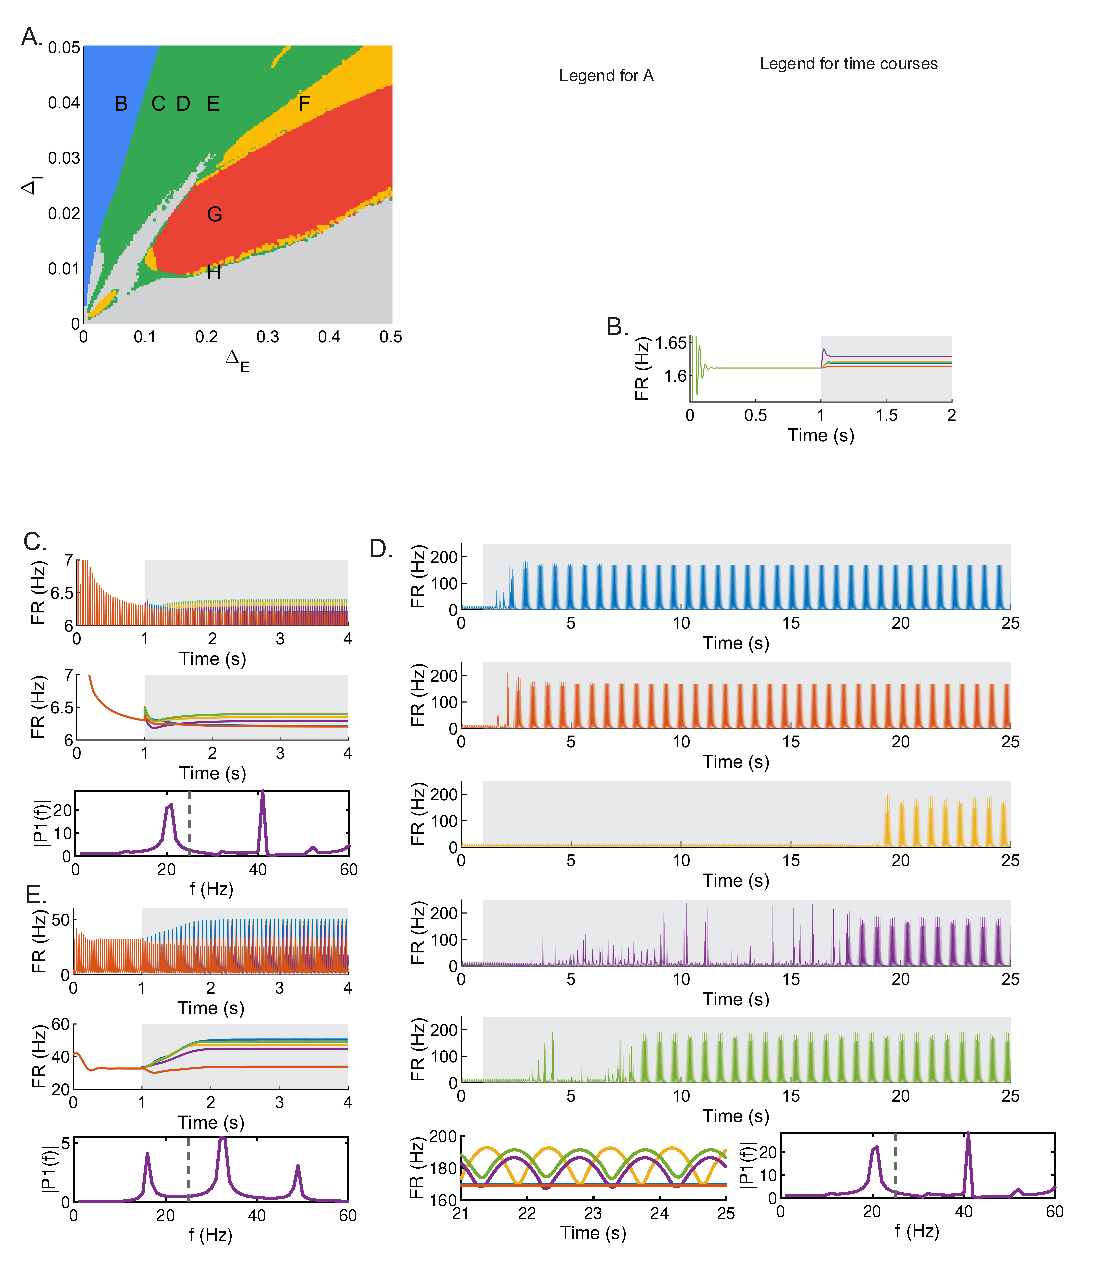
\includegraphics{Figure2.eps}
\begin{flushleft} {\bf Fig 2. Parameter plane analysis show different patterns of neuronal response.}
\textbf{A.} Parameter plane of $\Delta_{back}^{E}$ and $\Delta_{back}^{I}$. \textbf{B-H} Neuronal response with parameter settings corresponding to the location of letters marked on \textbf{A}. While \textbf{B} only shows the raw data of firing rate, \textbf{C}-\textbf{H} show raw data, envelope and amplitude spectrum of firing rate. The amplitude spectrum are obtained from the firing rate under condition S1S2+A1. Dash line in the amplitude spectrum denotes f=25(Hz). \textbf{B}: $\Delta_{back}^{E}=0.05$, $\Delta_{back}^{I}=0.04$, \textbf{C}: $\Delta_{back}^{E}=0.11$, $\Delta_{back}^{I}=0.04$, \textbf{D}: $\Delta_{back}^{E}=0.15$, $\Delta_{back}^{I}=0.04$, \textbf{E}: $\Delta_{back}^{E}=0.2$, $\Delta_{back}^{I}=0.04$, \textbf{F}: $\Delta_{back}^{E}=0.35$, $\Delta_{back}^{I}=0.04$, \textbf{G}: $\Delta_{back}^{E}=0.2$, $\Delta_{back}^{I}=0.02$, \textbf{H}: $\Delta_{back}^{E}=0.2$, $\Delta_{back}^{I}=0.0095$. 
\end{flushleft}
% \label{fig2}
\hypertarget{fig:fig2}{}
\end{adjustwidth}
\end{figure}

\subsection*{The winner-takes-all principle does not always hold and is effected by the inter-column connection}
The winner-takes-all principle means that for a multicolumnar structure with different excitability level, the more activated one will suppress the excitation of the others. In our study of two column paradigm, as \hyperlink{fig:fig3}{Fig 3A} shows, if Col1 is more activated than Col2, i.e. under condition S1 or S1S2+A1, the excitatory population in layer 2/3 of Col1 will activate the inhibitory population in layer 2/3 of Col2 more than the opposite pathway, which means the yellow pathway should be stronger than the magenta pathway. Due to the inhibitory population in Col2 is more activated than the one in Col1, it will inhibit the excitatory population in Col2 more than its counterpart do in Col1.
To investigate the winner-takes-all principle, we first define the pathway current from population Y to population X $C_{Y}^{X}$ in a period of time T as

\begin{eqnarray}
\label{eq:6}
    C_{Y}^{X} = \int_{0}^{T}(v_{syn}^{Y}-v_{X})^{2}g_{Y}^{X}P_{Y}^{X}dt,
\end{eqnarray}

where T is a time much longer than one period of oscillation. Here we set $T=???$. As to the free parameter $\Delta_{back}^{E}$ and $\Delta_{back}^{I}$, we focus on the parameter settings showing the ordered pattern which is the red region in \hyperlink{fig:fig2}{Fig 2A}. Surprisingly, we find that the winner-takes-all principle does not always hold and sometimes the opposite situation will occur that the less activated column exported larger pathway current to the activated column than its counterpart in the more activated column. \hyperlink{fig:fig3}{Fig 3B} shows the parameter settings agree or not agree with the winner-takes-all principle. Note that the yellow and magenta region together is equal to the red region in \hyperlink{fig:fig2}{Fig 2A}. \hyperlink{fig:fig3}{Fig 3C} shows the pathway current under each condition, and the parameter settings are corresponding to the position of plus and cross symbols on \hyperlink{fig:fig3}{Fig 3B}. For the position marked as cross symbol, under conditions S1 and S2, Col1 or Col2 dominate the inter-column pathways respectively. For condition S1S2, the pathway current $C_{1}^{2}$ and $C_{2}^{1}$ are equal. Moreover, for conditions S1S2+A1 and S1S2+A2, due to the excitatory effect of attention input, Col1 or Col2 re-dominate the inter-column pathways respectively. However, when it comes to the position marked as plus symbol on parameter plane, although the dominant pathways are same under conditions S1, S2 and S1S2, the excitation induced by attention result in opposite effects. For conditions S1S2+A1 and S1S2+A2, the less activated column Col2 exports more pathway current than the more activated column.

Finally, we want to investigate whether it is possible to turn situation from disagree with the winner-takes-all principle to become agree with such principle. We change the probability of inter-column connection $P_{inter}$ and find that the original situation disagree with the winner-takes-all principle now agreed. As \hyperlink{fig:fig3}{Fig 3D} showed, as the setting of plus symbol, when $P_{inter}$ is rather small, the more activated column Col1 export less pathway current than the less activated column Col2 ($C_{1}^{2} - C_{2}^{1} < 0$). However, when $P_{inter}$ is large enough ($P_{inter}>0.1649$), the more activated column Col1 dominate the inter-column pathways and export more current to the less activated column Col2. We checked the effect of $P_{inter}$ in the situation that winner-takes-all originally held, as the cross symbol. Increasing or decreasing $P_{inter}$ will change the difference of $C_{1}^{2}$ and $C_{2}^{1}$, but $C_{1}^{2}$ is always larger than $C_{2}^{1}$. We also confirmed that the change of $P_{inter}$ do not disrupt the ordered pattern of oscillation amplitude. As \hyperlink{fig:fig3}{Fig 3E} shows, for both parameter settings, although the firing rate become lower with the increasing of $P_{inter}$, the ordered pattern is always held.

% FIGURE 3
\begin{figure}[!h]
\begin{adjustwidth}{-2in}{0.3in} % Comment out/remove adjustwidth environment if table fits in text column.
\centering
% \hspace*{-1.836in}
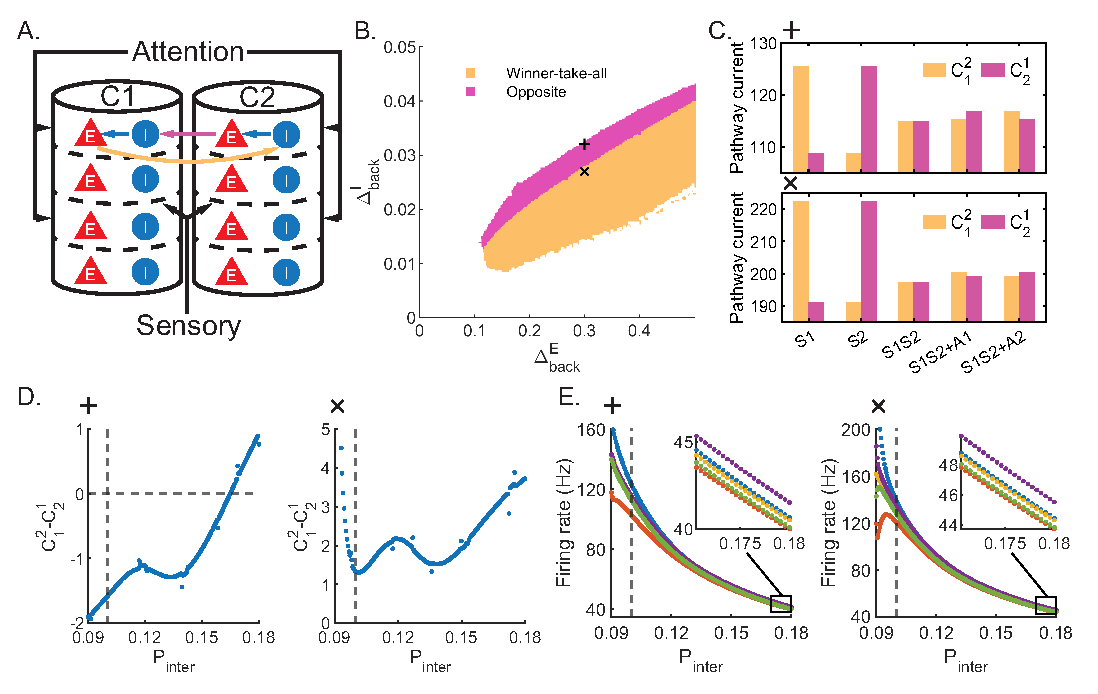
\includegraphics{Figure3.eps}
\begin{flushleft} {\bf Fig 3. Exception case of winner-takes-all principle.}
\textbf{A.} Parameter plane of $\Delta_{back}^{E}$ and $\Delta_{back}^{I}$. $\times$ and $+$ marks denote two parameter settings in the winner-takes-all region and opposite region respectively. $\times$: $\Delta_{back}^{E}=0.3$, $\Delta_{back}^{I}=0.027$; $+$: $\Delta_{back}^{E}=0.3$, $\Delta_{back}^{I}=0.032$. \textbf{B.} Structure of multicolumnar model highlighting the circuit among layer 2/3. \textbf{C.} Current in inter-column pathways under five conditions. \textbf{D.} Difference of two inter-column pathways with the change of connection probability of inter-column pathway $P_{inter}$ under condition S1S2+A1 The horizontal dash line denotes zero difference of two inter-column pathways. The vertical dash lines denote initial setting of the connection probability $P_{inter}=0.1$. \textbf{E.} Firing rate under five conditions with the change of connection probability of inter-column pathway $P_{inter}$. The vertical dash lines denote initial setting of the connection probability $P_{inter}=0.1$.
\end{flushleft}
% \label{fig3}
\hypertarget{fig:fig3}{}
\end{adjustwidth}
\end{figure}

\section*{Discussion}
summary our work

Nulla mi mi, venenatis sed ipsum varius, Table~\ref{table1} volutpat euismod diam. Proin rutrum vel massa non gravida. Quisque tempor sem et dignissim rutrum. 

\section*{Supporting information}

% Include only the SI item label in the paragraph heading. Use the \nameref{label} command to cite SI items in the text.

\paragraph*{S1 Appendix.}
\label{S1_Appendix}
{\bf Derivation of the mean-field approximation model} This appendix details the derivation from the QIF model Eq.~(\ref{eq:1}) to the mean-field apprximation model Eq.~(\ref{eq:4}).

\begin{eqnarray}
\label{eq:6}
    \frac{\partial}{\partial t}\rho_{X}(V_{X}|I_{X},t)=-\frac{\rho}{\rho V_{X}}\left[ \left( a_{X}V_{X}^{2} + b_{X}(t)V_{X} + c_{X}(t) + I_{X}\right) \rho_{X}(V_{X}|I_{X},t) \right],
\end{eqnarray}

\begin{eqnarray}
\label{eq:7}
    \rho_{X}(V_{X}|I_{X},t) = \frac{f(I_{X})}{\pi}\frac{x_{X}(I_{X},t)}{\left[ V_{X}-y_{X}(I_{X},t)\right]^{2} + x_{X}(I_{X},t)^{2}},
\end{eqnarray}

\begin{eqnarray}
\label{eq:8}
    \frac{d}{dt}x_{X}(I_{X},t) = 2a_{X}x_{X}(I_{X},t)y(I_{X},t) + b_{X}(t)x_{X}(I_{X},t),
\end{eqnarray}

\begin{eqnarray}
\label{eq:9}
    \frac{d}{dt}y_{X}(I_{X},t) = -a_{X}(x_{X}(I_{X},t)^{2} + a_{X}y_{X}(I_{X},t)^{2} + b_{X}(t)y_{X}(I_{X},t) + c_{X}(t) + I_{X},
\end{eqnarray}

\begin{eqnarray}
\label{eq:10}
    \frac{d}{dt}\omega_{X}(I_{X},t) = ia_{X}\omega_{X}(I_{X},t)^{2} + b_{X}(t)w_{X}(I_{X},t) + c_{X}(t) + I_{X},
\end{eqnarray}

\begin{eqnarray}
\label{eq:11}
    \frac{d}{dt}\omega_{X}(I_{X},t) = ia_{X}\omega_{X}(I_{X},t)^{2} + b_{X}(t)w_{X}(I_{X},t) + c_{X}(t) + I_{X},
\end{eqnarray}

\paragraph*{S2 Appendix.}
\label{S2_Appendix}
{\bf Simulation of the multicolumnar model} All the simulations are integrated by the Euler method, with a time step $\Delta t=0.01 (ms)$, using MATLAB (R2022b, https://www.mathworks.com/products/matlab.html). The code is available at https://github.com/Shawnzty/multicolumn.

\section*{Acknowledgments}
KAKENHI, JSPS?

\nolinenumbers

% Either type in your references using
% \begin{thebibliography}{}
% \bibitem{}
% Text
% \end{thebibliography}
%
% or
%
% Compile your BiBTeX database using our plos2015.bst
% style file and paste the contents of your .bbl file
% here. See http://journals.plos.org/plosone/s/latex for 
% step-by-step instructions.
% 
\begin{thebibliography}{10}

\bibitem{bib1}
Wagatsuma N, Potjans TC, Diesmann M, Fukai T.
\newblock {Layer-dependent attentional processing by top-down signals in a visual cortical microcircuit model}.
\newblock Front Comput Neurosci. 2011;5. doi: 10.3389/fncom.2011.00031 PMID: 21779240

\bibitem{bib2}
Ott E, Antonsen TM.
\newblock {Low dimensional behavior of large systems of globally coupled oscillators}.
\newblock Chaos. 2008; 18(3):037113. https://doi.org/10.1063/1.2973816 PMID: 19045487

\bibitem{bib3}
Montbrió E, Pazó D, Roxin A.
\newblock {Macroscopic description for networks of spiking neurons}.
\newblock Phys Rev X. 2015; 5(2):021028.

\bibitem{Mountcastle1957}
Mountcastle, Vernon
\newblock  {Modality and topographic properties of single neurons of cat's somatic sensory cortex}.
\newblock J Neurophysiol. 1957; 20 (4): 408–34. doi:10.1152/jn.1957.20.4.408 PMID 13439410.

\bibitem{hubel1959}
Hubel DH, Wiesel TN.
\newblock {Receptive fields of single neurones in the cat's striate cortex}.
\newblock J Physiol. 1959; 148: 574-591. doi: 10.1113/jphysiol.1959.sp006308 PMID: 14403679.

\bibitem{reynolds1999}
Reynolds JH, Chelazzi L, Desimone R.
\newblock {Competitive Mechanisms Subserve Attention in Macaque Areas V2 and V4}.
\newblock J Neurosci. 1999; 19 (5): 1736-1753. doi: 10.1523/JNEUROSCI.19-05-01736.1999 PMID: 10024360.

\bibitem{luck1997}
Luck SJ, Chelazzi L, Hillyard SA, Desimone R.
\newblock {Neural mechanisms of spatial selective attention in areas V1, V2, and V4 of macaque visual cortex}
\newblock J Neurophysiol. 1997; 77(1): 24-42. doi: 10.1152/jn.1997.77.1.24. PMID: 9120566.


\end{thebibliography}
\end{document}

